\documentclass[xcolor=svgnames,17pt]{beamer}

\usepackage[export]{adjustbox}
\usepackage{bashful}
\usepackage{bookmark}
\usepackage{colortbl} \arrayrulecolor[gray]{0.7}
\usepackage{microtype}
\usepackage{pgfpages}
\usepackage{rotating}
\usepackage{textcomp}
\usepackage{tabularx}
\usepackage{xspace}
\usepackage{verbatim}

\usepackage{fontspec}

\hypersetup{hidelinks,pdfpagemode=}

\urlstyle{same}

\newcommand*{\sizefont}[1]{%
    \ifcase#1\relax
    \or \tiny
    \or \scriptsize
    \or \footnotesize
    \or \small
    \or \normalsize
    \or \large
    \or \Large
    \or \LARGE
    \or \huge
    \or \Huge
    \fi}

%%

\newcommand*{\mybullet}{\tikz[baseline=-.6ex]\node[%
    draw,circle,inner sep = -0.15ex,fill]{.};\xspace}

%\setbeamertemplate{footline}{
%    \usebeamercolor[fg]{page number in head/foot}%
%    \usebeamerfont{page number in head/foot}%
%    \hspace*{1ex}\insertframenumber\,/\,\inserttotalframenumber\hfill
%    github.com/andrewdotn/...\ }

\newcommand*{\plainfooter}{%
    \setbeamertemplate{footline}{
        \usebeamercolor[fg]{page number in head/foot}%
        \usebeamerfont{page number in head/foot}%
        \hspace*{1ex}\insertframenumber\,/\,\inserttotalframenumber\vskip2pt}}

\makeatletter
\def\alphslide{\@alph{\intcalcAdd{1}{\intcalcSub{\thepage}{\beamer@framestartpage}}}}
\newcommand*{\plainstepfooter}{
    \setbeamertemplate{footline}{
        \usebeamercolor[fg]{page number in head/foot}%
        \usebeamerfont{page number in head/foot}%
        \hspace*{1ex}\insertframenumber\alphslide\,/\,\inserttotalframenumber\vskip2pt}}
\makeatother

\setbeamertemplate{note page}{
    \sizefont{3}
    \setlength{\parskip}{10pt}
    \insertnote
    \par}

\setbeamertemplate{navigation symbols}{}
\setbeamerfont{title}{size=\LARGE}
\setbeamerfont{frametitle}{size=\LARGE}
\setbeamerfont{framesubtitle}{size=\normalsize}

\newcommand*{\tocsection}[1]{\pdfbookmark[2]{#1}{#1}}

\lstdefinestyle{bashfulStdout}{
    basicstyle=\ttfamily,
    keywords={},
    showstringspaces=false
}%

%%

\title{Dates, times, \\ and timezones: \\ Python vs the real world}

\author{\texorpdfstring{%
    Andrew Neitsch}{Andrew Neitsch}}

\date{\small 2017-09-28}

\begin{document}

\tocsection{Title page}

\sizefont{4}

\begin{frame}[plain]
\titlepage
\end{frame}

\begin{frame}{Outline}
\tableofcontents
\end{frame}

\section{Introduction}

\def\fillinblank{\_\_\_\_}

\begin{frame}{Basic use cases for date and time computation}
\begin{itemize}
\item What time is it now?
\item What time is it in \fillinblank?
\item What time is here when it’s \fillinblank in \fillinblank?
\item What does the date 9/10/11 mean?
\item How long ago did \fillinblank happen?
\item Remind me when \fillinblank is about to happen
\end{itemize}
\end{frame}

\section{Theory}

\begin{frame}
\tableofcontents[currentsection]
\end{frame}

\begin{frame}{Dates and times for humans}

\begin{itemize}
\item Times
\item Dates
\item Time zones
\end{itemize}

\end{frame}

\begin{frame}{Times for humans}
\begin{itemize}
\item \alert{Times}

Pretty straightforward

Partition the day into regular intervals:

\only<2->{24 hours of 60 minutes of 60 seconds}
\item Dates
\item Time zones
\end{itemize}
\end{frame}

\begin{frame}[fragile]{Dates for humans}
\begin{itemize}
\item Times
\item \alert{Dates}

\only<1-2>{Partition the day into \textit{irregular} intervals}

\only<2->{12 months of varying lengths}

\only<2->{Pattern depends on year}

\item Time zones
\end{itemize}
\end{frame}

\begin{frame}[fragile]{Dates for humans}
\begin{itemize}
\item Times
\item \alert{Dates} \\
    Partition the day into \textit{irregular} intervals

    Root problem: \\
    365.24220 earth rotations per orbit of sun

\bash[stdout,script,prefix=$\space]
gfactor 365
\END

Not a convenient number, \\
so months of varying lengths

\item Time zones
\end{itemize}
\end{frame}

\begin{frame}[fragile]{Dates for humans}
\begin{itemize}
\item Times
\item \alert{Dates}

    365.24220 earth rotations per orbit of sun

    Leap days to deal with the fractional part

{
\sizefont{2}
\bash[stdout]
echo '
3 / ((365 + 1/4 - 1/100 + 1/400) - 365.24220)
' | ./python-interpret
\END
}

\item Time zones
\end{itemize}
\end{frame}

\begin{frame}{Time zones for humans}

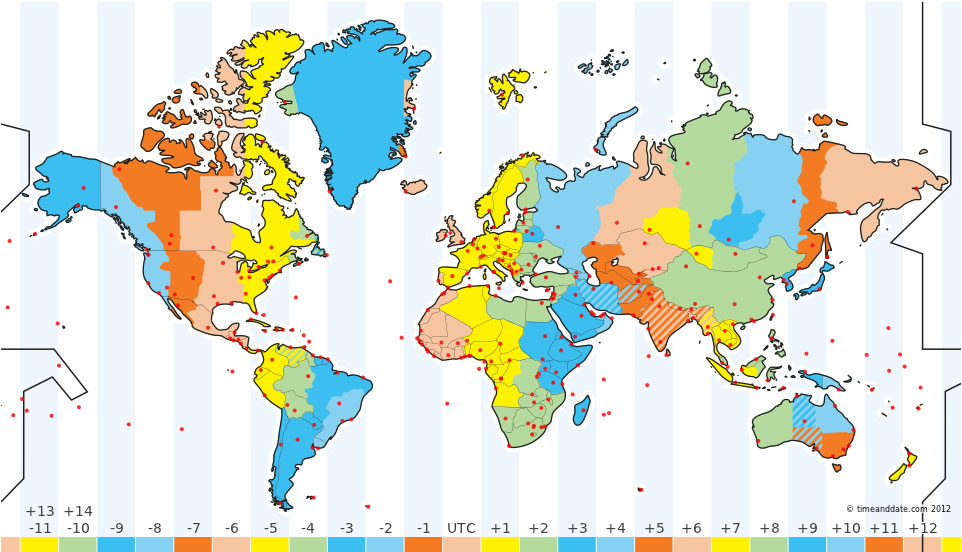
\includegraphics[width=\paperwidth,center]{timezonemapdateline.jpg}

\end{frame}

\begin{frame}{Time zones for humans}

\begin{itemize}

\only<1>{
\item Noon is slightly different in different parts of the world
}

\only<2>{
\item Time zones are a balance between precision of having clocks close to
the sun, and the convenience of uniform time over large parts of the earth
}

\only<3->{
\item Defined by local laws, can change with little or no notice
}

\only<4->{
\item Defined relative to Universal Coordinated Time: UTC
}
\only<4>{(Similar to historical Greenwich Mean Time)}

\only<5-6>{
\item Today, Calgary is UTC-0600, which means exactly 6 hours behind UTC
}

\only<6>{
\item Changes to UTC-0700 at 2:00 a.m. on November 5
}

\only<7>{
\item Egypt 2014: Daylight savings transitions in May, June, July, and September
}

\only<8>{
\item Not a lot of theory here: just need to be able to look it up
}

\end{itemize}

\end{frame}

\begin{frame}{Time zones for humans}

You can’t know how far away a date or time is from any other date or time
without knowing what timezones they are referring to \\[\baselineskip]

\pause

Given that time is what keeps everything from happening at once ...
\\[\baselineskip]

\pause

That’s pretty important.

\end{frame}

\begin{frame}{Conclusions for humans}

\begin{itemize}
\item Times

\only<1->{
Divided into regular intervals, relatively straightforward
}

\item Dates

\only<2->{
Divided into irregular intervals, complicated but unchanging
}

\item Time zones

\only<3->{
Super-complicated, arbitrary,
subject to change without notice
}

\end{itemize}

\only<4>{
Time and date are meaningless without timezone
}

\end{frame}

\begin{frame}{Dates and times for computers}

Computers do not care about what we care about

\pause

\begin{itemize}
\item \alert<1-2>{Times}

\begin{onlyenv}<2-3>
We can just count seconds since some arbitrary point

Do math by subtracting
\end{onlyenv}

\only<3>{
Seconds since start of January 1, 1970, UTC: 1506624282
}

\item \alert<4>{Dates}
\item \alert<4>{Time zones}

\only<4>{Only matter for I/O with humans}

\end{itemize}

\end{frame}

\begin{frame}{Theoretical conclusions}

Huamns and computers have very different needs when it comes to dates and
times

\end{frame}

\section{Python}

\begin{frame}{Basic use cases for date and time computation}
\begin{itemize}
\item What time is it now?
\item What time is it in \fillinblank?
\item What time is here when it’s \fillinblank in \fillinblank?
\item What does the date 9/10/11 mean?
\item How long ago did \fillinblank happen?
\item Remind me when \fillinblank is about to happen
\end{itemize}
\end{frame}

\begin{frame}
\tableofcontents[currentsection]
\end{frame}

\begin{frame}[fragile]{Python's standard library}

Create datetime objects and convert them to seconds since the epoch:

\pause

{\sizefont{3}
\bash[stdout]
echo '
datetime.datetime.utcnow().strftime("%s")


datetime.datetime.now().strftime("%s")
' | ./python-interpret
\END
}

\pause

\begin{onlyenv}<3>
This is substantially more dangerous than using MySQL:

\sizefont{2}
\begin{verbatim}
mysql> SELECT 0 = 'banana';
+--------------+
| 0 = 'banana' |
+--------------+
|            1 |
+--------------+
1 row in set, 1 warning (0.00 sec)
\end{verbatim}
\end{onlyenv}

\pause

\alert{Python’s standard library does not understand time zones and is not
generally safe to use for date or time computations.}

\end{frame}

\section{Pendulum}

\begin{frame}
\tableofcontents[currentsection]
\end{frame}

\begin{frame}{Pendulum: “Python datetime made easy”}
\texttt{pip3 install pendulum}
\end{frame}

\begin{frame}[fragile]{What time is it now?}

{\sizefont{3}
\bash[stdout]
echo '
now = pendulum.now()


now


now.timezone


now.timestamp()


now.day_of_week == pendulum.THURSDAY
' | ./python-interpret
\END
}

\pause

{\sizefont{3}
\bash[stdout]
echo '
utcnow = pendulum.utcnow()


utcnow


utcnow.timestamp()
' | ./python-interpret
\END
}

\end{frame}

\section{Conclusions}

\begin{frame}
\tableofcontents[currentsection]
\end{frame}

\begin{frame}{What we haven’t talked about}

Pendulum may or not help you here; you’re on your own.

\pause

\begin{itemize}
\item Other calendars: Buddhist, Coptic, Hebrew, Islamic ...
\item Localization
\item Leap seconds
\item Time synchronization
\item ...
\end{itemize}
\end{frame}

\begin{frame}{Conclusion}
\begin{itemize}
\item Dates and times are most complicatied because of time zones
\item Python falls down hard there
\item Pendulum handles common date, time, and time zone computations in an
easier and safer way
\end{itemize}
\end{frame}

\end{document}
